\section{Implementación}

El método requiere de los siguientes datos de entrada:
\begin{description}
\item[divisions] cantidad de divisiones sobre la cuál se colocarán los picos.
\item[nroPeaks] cantidad total de picos.
\item[yMin] altura mínima permitida de un pico.
\item[yMin] altura máxima permitida de un pico.
\item[ruggedness] escabrosidad del terreno, es decir, qué tanto afecta un pico a sus posiciones aledañas.
\end{description}
\smallskip

Lo que denominamos '\textbf{pico}', es un valor que será generado y ubicado aleatoriamente ocupando alguna de las posiciones posibles (divisions). Representa un punto de elevación en el terreno que luego el algoritmo se encargará de interpretar (en conjunto con la información del resto de los picos) para definir el valor definitivo que tendrá la elevación en cada punto del terreno.
\begin{figure}[h]
\centering
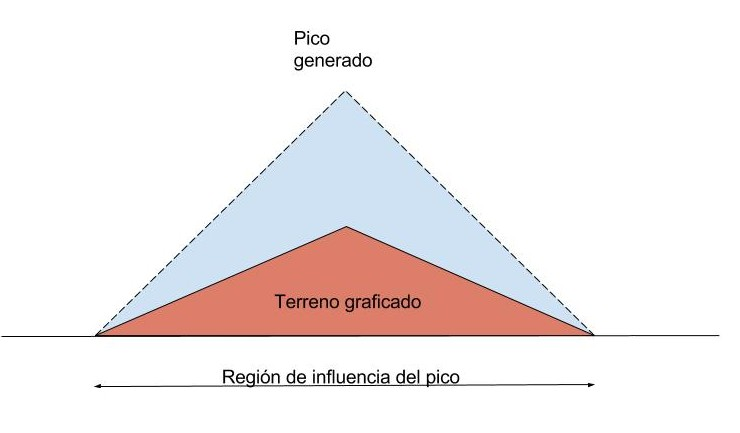
\includegraphics[width=0.7\linewidth]{imagenes/Pico1}
\caption{}
\label{fig:Pico1}
\end{figure}
\begin{figure}[h]
	\centering
	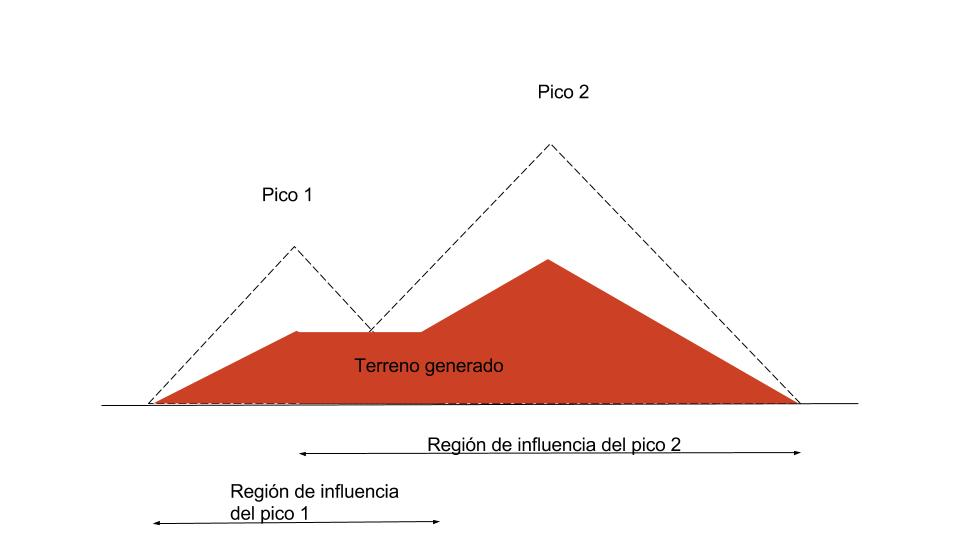
\includegraphics[width=0.7\linewidth]{imagenes/pico2}
	\caption{}
	\label{fig:pico2}
\end{figure}

En la figura 1 podemos ver un terreno generado a partir de un único pico, como se puede apreciar el valor del pico se promedia con el suelo para obtener el terreno definitivo. Se observa también una zona de influencia del pico, es aquella en la cual el punto de elevación afecta en el cálculo final del terreno.


El concepto de '\textbf{influencia}' de un pico podemos visualizarlo mejor en la figura 2. El terreno fue generado a partir de dos picos, existe una región  donde tenemos influencia por parte de ambos, es donde se forma una meseta ya que el algoritmo promedia la altura que tienen los picos en esa región. En el resto del terreno hay influencia de un sólo pico o ninguno.

En nuestro caso también contamos con las siguientes entradas, las cuáles agregamos por razones de utilidad a la hora de experimentar y comparar las implementaciones de C y ASM.
\begin{description}
\item[seed] permite setear una semilla particular para el random, esto es para lograr el mismo gráfico y poder experimentar con datos más certeros.
\item[debugging] si una semilla es proporcionada entonces se le puede decir al programa que entre en modo verbouse; el cuál nos va a dar, además del gráfico, el valor numérico de cada posición del terrreno final y la posición y tamaño original de cada pico.
\end{description}
\smallskip

Para poder llevar a cabo el método vamos a estar utilizando las siguientes estructuras:
\begin{description}
\item[peaksPos] arreglo con nroPeaks posiciones, cada una contiene la posición dentro del terreno de dicho pico. Las posiciones van de 0 a divisions-1.
\item[peaksSize] arreglo con nroPeaks posiciones, cada una contiene la altura de dicho pico. Las alturas posible están entre yMin e yMax (inclusive en ambos casos).
\item[terrain] vector con los valores numéricos finales de cada posición del terreno.
\end{description}
\smallskip

Los picos son generados de manera aleatoria, tanto su posición como su altura (dentro de los límites explicados más arriba). Luego se hace lo siguiente:

\begin{algorithm}
\begin{algorithmic}

\ForAll{divisions} 
	\ForAll{peaks} 
		\Comment{se calcula la influencia de cada pico para cada posición}
		\State influencia $\gets$ altura del pico - distancia del pico a la posición actual * ruggedness.
	\EndFor
	
	\If{la posición no tiene influencia de nadie} 
		\State valor final de la posición $\gets$ 0.
	
	\ElsIf{la posición solo es influenciada por un pico} 
		\State valor final de la posición $\gets$ influencia / 2.
	
	\ElsIf{la posición es influenciada por dos o más picos}
		\State valor final de la posición $\gets$ influencia / cantidad de picos con influencia sobre ella.
		
	\EndIf

\EndFor

\end{algorithmic}
\end{algorithm}

Quedando así en cada posición del terreno final el valor de 'promediar' todos los picos que tienen influencia sobre ella.

La complejidad teórica del algoritmo es $\theta(divisions*peaks)$ ya que indefectiblemente se recorren ambos y el resto de las operaciones son $O(1)$.

\subsection{Versión de C}
Está versión es muy sencilla ya que se puede mapear directamente el pseudocódigo a código, con pocas modificaciones. Luego basta con compilar utilizando las mejoras de sse para contar con las herramientas de SIMD.

\subsection{Versión de ASM}
La idea es simple, recorrer las posiciones del terreno de a cuatro, ya que como cada una es un float esa es la cantidad que entran en un registro xmm. 
Luego, en cada iteración, recorrer todos los picos, también de a cuatro (son int pero de 32 bits, es decir, cuatro por registro xmm).

Cuando obtenemos los datos de los picos, expandimos y repetimos la información de cada uno en distintos registros. 
Para que la explicación sea más clara mostraremos el caso del pico uno (P1) siendo los demás prácticamente iguales salvo por la información a usar. Entonces:\\

Primero se replica la posición actual en un registro xmm, al cuál le sumamos un registro constante con los enteros 0 a 3, es decir, nos queda el valor de cada una de las cuatro posiciones que estamos calculando en cada entero.

\begin{center}
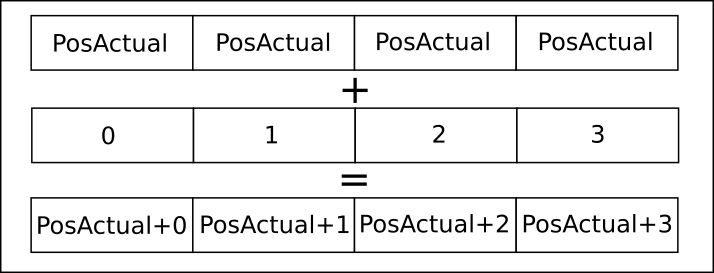
\includegraphics[scale=0.5]{imagenes/posActual.png} 
\end{center}

Luego, tanto para la posición (Pos) como para la altura (Size) de P1, se crean registros con la información replicada en cada int.

\begin{center}
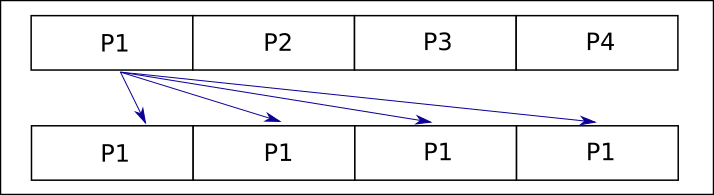
\includegraphics[scale=0.5]{imagenes/P1replicaInfo.png} 
\end{center}

Contamos con dos acumuladores, uno para la 'influencia' de los picos en esa posición y otro para la cantidad de picos que influyen. Para calcular el primero realizamos lo siguiente, donde Abs hace referencia a la función de valor absoluto:

\begin{center}
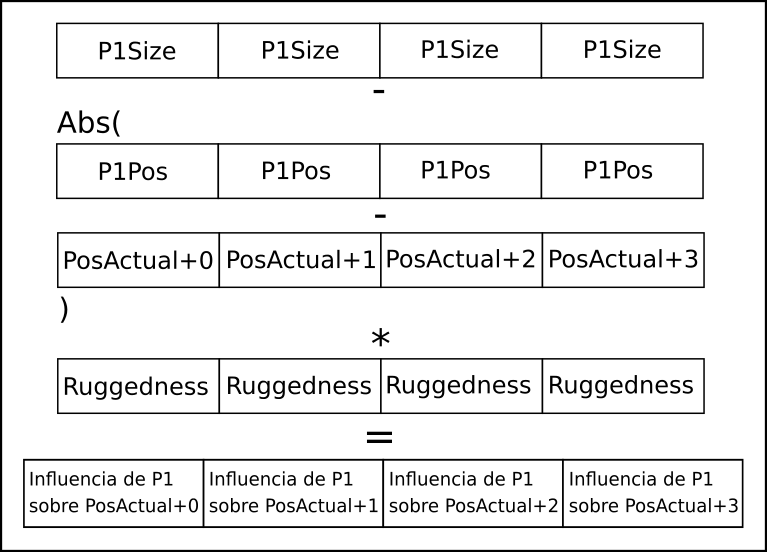
\includegraphics[scale=0.5]{imagenes/calculoInfluencia.png} 
\end{center}

Utilizando el registro que contiene la influencia obtenemos si el pico influye (influencia $>$ 0) o no (caso contrario) sobre cada una de las cuatro posiciones.

Sumando esta información para cada pico obtenemos cuánta influencia, y de cuántos picos, tiene una posición determinada. Así al final del ciclo que recorre los picos solo nos queda dividir influencia por cantidad de picos y así obtenemos el valor real del terreno en la posición.
